\subsection{Considerações Práticas}

Embora o modelo apresentado seja conceitualmente simples, sua implementação prática depende diretamente do controle preciso do atraso $\Delta t$.

Para que o detector funcione corretamente, o atraso deve ser suficientemente pequeno para garantir que o pulso gerado seja curto, mas suficientemente grande para que exista uma diferença detectável entre $clk$ e $clk_{delay}$. Caso $\Delta t$ seja muito grande, o circuito pode gerar pulsos indesejados ou múltiplas ativações.

Além disso, variações no atraso de propagação dos componentes podem introduzir incertezas temporais, afetando a precisão da detecção de borda. Em sistemas reais, esse fenômeno está relacionado ao \textit{jitter} e ao \textit{skew} do clock.

Em ambientes discretos, como no Logisim ou em circuitos de Redstone, o atraso é quantizado, o que simplifica a análise, mas impõe limitações na resolução temporal do detector.

Apesar dessas restrições, detectores de borda são amplamente utilizados como mecanismos fundamentais para sincronização, sendo responsáveis por converter transições de nível em eventos discretos que podem ser utilizados por máquinas de estado e circuitos sequenciais.

Por exemplo, no Minecraft, para solucionar o problema do tamanho do pulso de retomada das oscilações, pode-se utilizar um detector de borda de subida no bit $A$. Dessa forma, quando ocorre uma transição $A_t = 0$ para $A_{t+1} = 1$. Tal pulso possui duração aproximadamente igual ao atraso $\Delta t$, garantindo que sua largura seja mínima e controlada, evitando a geração de múltiplos pulsos no circuito.

\begin{figure}[H]
    \centering
    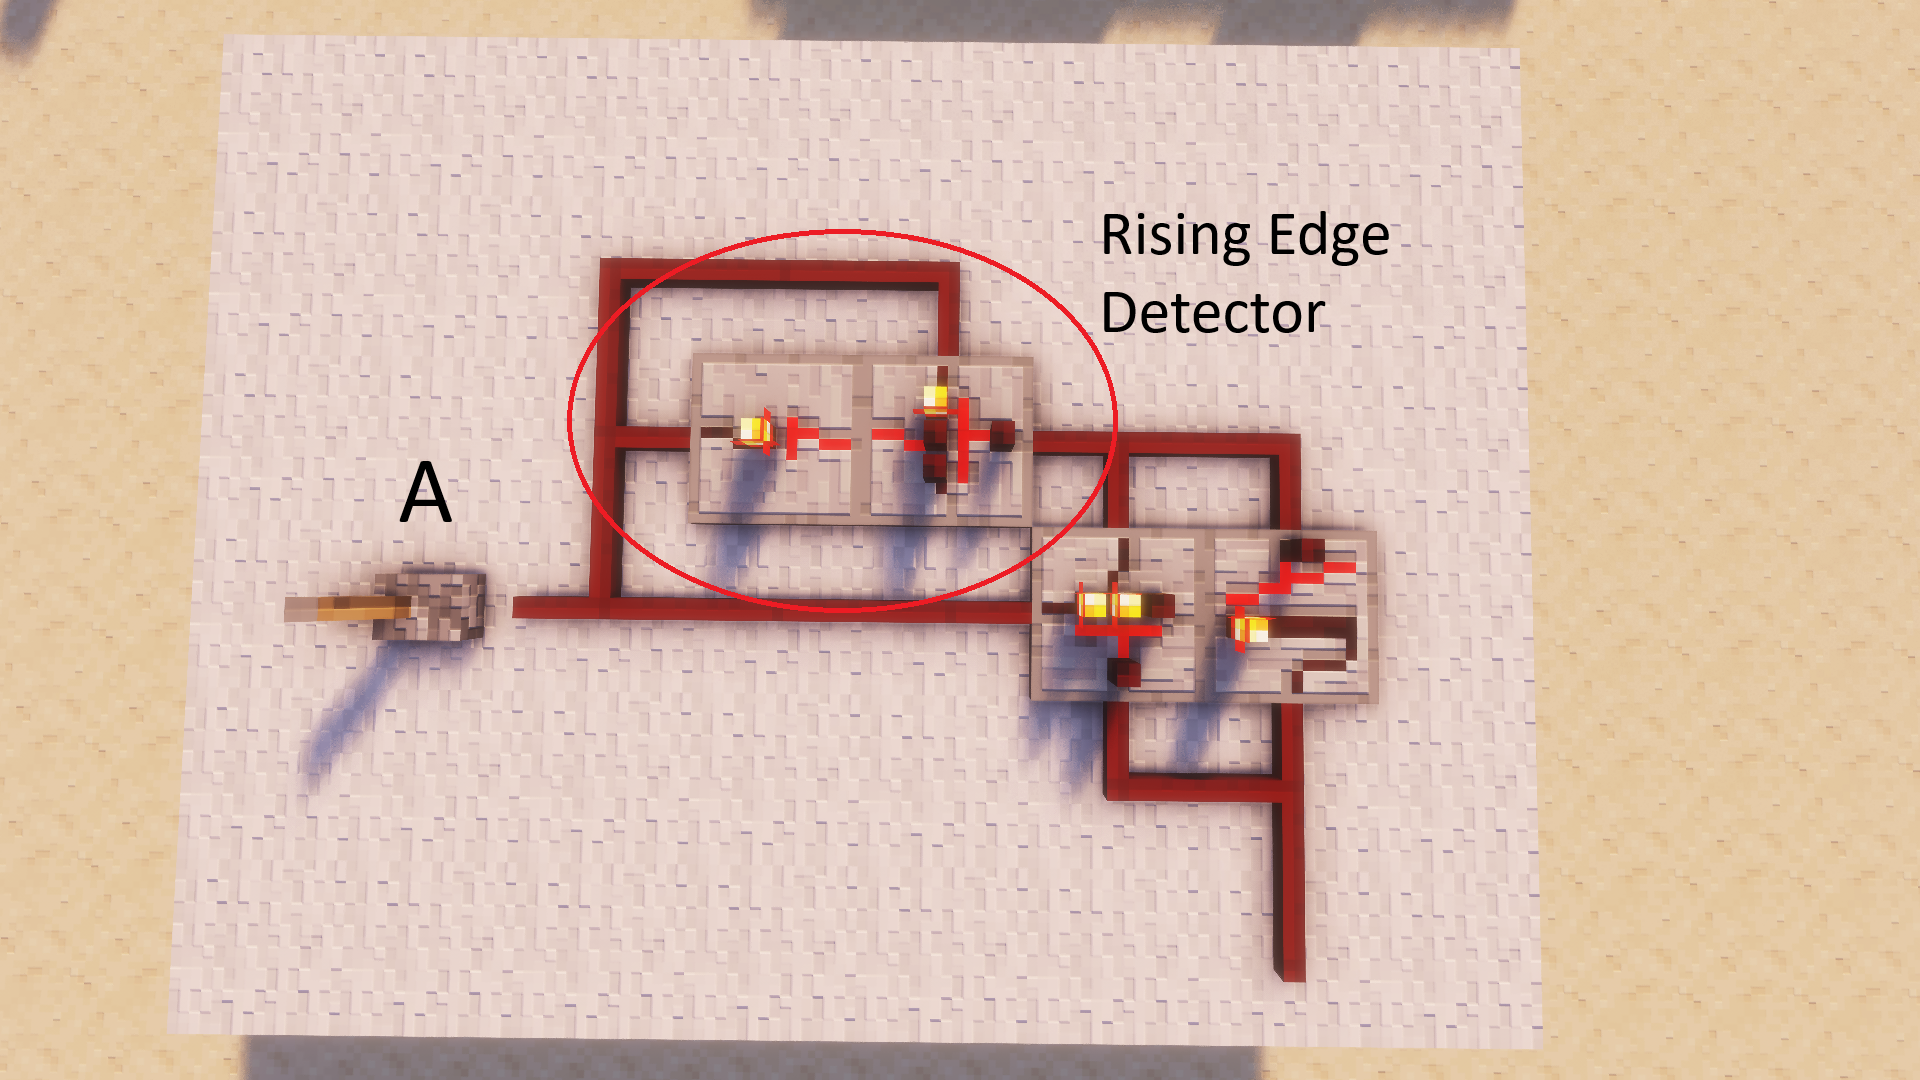
\includegraphics[width=0.8\linewidth]{images/toggle-redstone-clock.png}
    \caption{Clock on/of de redstone}
    \label{fig:toggle-redstone-clock}
\end{figure}

A título de curiosidade, existem tecnologias que exploram simultaneamente as bordas de subida e de descida do clock para realizar operações de leitura e escrita de dados. Essas tecnologias são conhecidas como \textit{Double Data Rate} (DDR).

Em sistemas DDR, os dados são transferidos duas vezes por período de clock: uma vez na borda de subida e outra na borda de descida. Dessa forma, para uma mesma frequência de clock $f$, obtém-se uma taxa efetiva de transferência equivalente a $2f$.

Essa abordagem permite aumentar o desempenho do sistema sem a necessidade de elevar a frequência do clock, o que é particularmente vantajoso devido às limitações físicas associadas a altas frequências, como maior consumo de energia, dissipação térmica e efeitos de propagação.